{\color{blue}
\section{Ablation Study}

To isolate the impact of memory-plane features on the kernels, we conduct an ablation study extending the OE baseline with selected DISCO-inspired attributes. The measurements compare OE configurations and do not represent a comparison of the complete DISCO and OE architectures.

On the memory plane, DISCO has the SPM, the VWRs and an Scalar Register File shared among the PEs in a column.  

\subsection{Impact of the Scalar Register File}
\label{subsec:srf-ablation}

The experimental OE extension provides eight scalar registers shared by the
RCs in each column and initialized before kernel execution. The \emph{SRF
Offsets} mapping stores combined address increments and reused parameters in
these registers; the \emph{SRF Base} mapping stores reusable base addresses
for restoring matrix positions during traversal. Both use the same 4$\times$4
CGRA and the same SRF capacity.

Figure~\ref{fig:srf-ablation} summarizes the measured speedups. Total
simulated cycles include the model's static instruction-configuration cost
and executed kernel cycles.

\begin{figure}
    \centering
    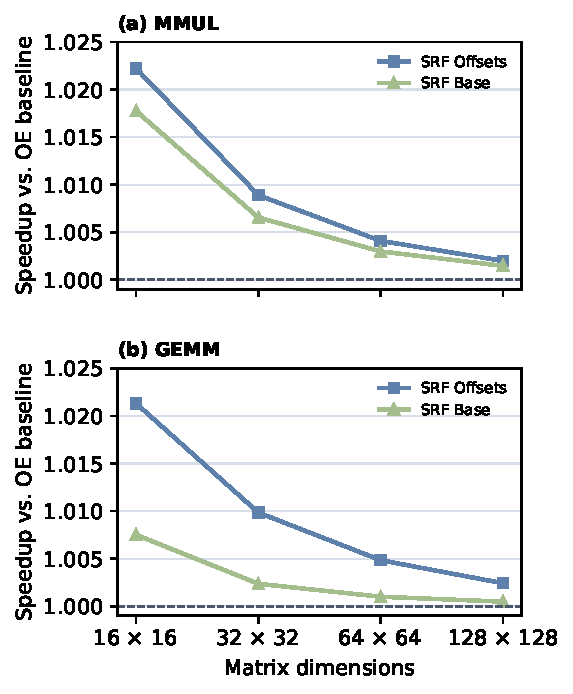
\includegraphics[width=\linewidth]{Figures/srf_ablation.pdf}
    \caption{Speedup over the original OE mapping for (a) MMUL and (b) GEMM.
    The horizontal dashed line denotes the OE baseline (1$\times$).}
    \label{fig:srf-ablation}
\end{figure}

All 24 executions matched their independent CPU references for every
matrix element, using identical deterministic inputs across versions at each
size. For MMUL, SRF Offsets reduces total cycles by 101, 305, 1,097, and 4,217
cycles for sizes 16, 32, 64, and 128, respectively (speedups of 1.0222, 1.0089,
1.0041, and 1.0020$\times$). SRF Base saves 81, 225, 801, and 3,105 cycles
(1.0178, 1.0065, 1.0030, and 1.0015$\times$). Offsets is the faster mapping
at every size. Its absolute savings grow with the number of output tiles,
while its percentage benefit declines as matrix multiplication work grows.

GEMM computes $C=\alpha AB+\beta C$ with $\alpha=125$ and $\beta=14$.
SRF Offsets saves 112, 364, 1,348, and 5,236 cycles across the same sizes,
for speedups of 1.0213, 1.0098, 1.0048, and 1.0024$\times$. SRF Base saves
40, 88, 280, and 1,048 cycles (1.0075, 1.0024, 1.0010, and 1.0005$\times$).
The fused Offsets schedule removes three further PCs relative to the prior
Offsets mapping (12 configuration cycles); its total-cycle reductions over
that mapping are 88, 292, 1,084, and 4,204 cycles, of which 76, 280, 1,072,
and 4,192 are executed-kernel cycles. Thus, the new fusion produces larger
absolute savings for GEMM than MMUL at each size, although MMUL has a slightly
larger relative gain at 16$\times$16. In both kernels, sharing scalars and
combined strides reduces configuration and address-management work, while
the unchanged matrix computation dominates at larger sizes. This result
characterizes the SRF extension on the OE mapping and does not imply a
whole-architecture performance comparison.

Per-run commands, input hashes, and validated cycle totals are recorded in
\texttt{paper/srf\_ablation\_results.csv} and
\texttt{paper/gemm\_srf\_ablation\_results.csv}; the plotted speedups can be
reproduced with \texttt{paper/plot\_srf\_ablation.py}.
}
